\documentclass[preprint,12pt]{elsarticle}

\usepackage{amsfonts,amssymb,amsmath}
\usepackage{amsthm}
\usepackage{bm}
\usepackage{graphicx}
\usepackage{svg}
\usepackage[caption=false]{subfig}
\usepackage{enumerate}

\usepackage{dcolumn}
\usepackage{bm}
\usepackage{color}
\usepackage{epsfig}
\usepackage{multirow}
\usepackage{mathrsfs}
\usepackage{hyperref}
\usepackage{cleveref}
\usepackage{epstopdf}
\usepackage{subcaption}
\usepackage{autobreak}
\usepackage{tikz}
\usepackage{placeins}
\usepackage{float}
\usepackage{algorithm}
\usepackage{algpseudocode}

\sloppy

% math commands
\newcommand{\V}[1]{\boldsymbol{#1}}
\newcommand{\T}[1]{\text{#1}}
\newcommand{\M}[1]{\boldsymbol{#1}}
\newcommand{\Set}[1]{\mathbb{#1}}
\newcommand{\D}[1]{\Delta#1}
\renewcommand{\d}[1]{\delta#1}
\newcommand{\norm}[1]{\left\Vert #1\right\Vert }
\newcommand{\abs}[1]{\left|#1\right|}
\newcommand{\av}[1]{\left\langle #1\right\rangle }
\newcommand{\sM}[1]{\M{\mathcal{#1}}}
\newcommand{\dprime}{\prime\prime}
\renewcommand{\i}{\mathrm i}
\newcommand{\follows}{\quad\Rightarrow\quad}
\newcommand{\eqd}{\overset{d}{=}}
\newcommand{\spe}[1]{\mathscr{#1}}
\newcommand{\eps}{\varepsilon}
\newcommand{\mrm}[1]{\mathrm{#1}}
\newcommand{\te}[1]{\text{#1}}
\providecommand{\grad}{}
\renewcommand{\grad}{\nabla}
\newcommand{\R}{\mathbb{R}}
\newcommand{\rhob}{\bm{\rho}}
\newcommand{\xib}{\bm{\xi}}
\newcommand{\phihat}{\widehat{\phi}}
\newcommand{\PV}{\operatorname{PV}}

\newtheorem{theorem}{Theorem}[section]
\newtheorem{proposition}[theorem]{Proposition}
\newtheorem{remark}[theorem]{Remark}

\begin{document}

\begin{frontmatter}

\title{Adaptive Boundary-Integral Computation of Screened Coulomb Integrals in Dielectric Environments}

\author[aff1]{author1}
\ead{email1}

\address[aff1]{aff1}

\begin{abstract}
This is an abstract.
\end{abstract}

\begin{keyword}
% Poisson equation \sep dielectric interface \sep boundary integral equation
\end{keyword}

\end{frontmatter}

\section{Introduction}

% This is an introduction~\cite{BarnettGreengard2010}.

In this work, we focus on developing a numerical solver for evaluating the four-indices integrals~\cite{cramer2013essentials} of the form
\begin{equation}\label{eq:four_indices}
    \begin{split}
    V_{ijkl} &= \iint \varphi_i(x_1)\varphi_j^*(x_1)\, K(x_1,x_2)\,
        \varphi_k(x_2)\varphi_l^*(x_2)\, \mathrm{d}x_1\mathrm{d}x_2\\
    &= \int \rho_{ij}(x_1)\, K(x_1,x_2)\, \rho_{kl}(x_2)\, \mathrm{d}x_1\mathrm{d}x_2\\
    &= \int \rho_{ij}(x_1)\, \phi_{kl}(x_1)\, \mathrm{d}x_1,
    \end{split}
\end{equation}
where~$\{\varphi_i\}$ are a set of basis functions, $\rho_{ij}(x) = \varphi_i(x)\varphi_j^*(x)$ is the source density, $K(x_1,x_2)$ is the Green's function of the Poisson equation in the presence of dielectric interfaces, and $\phi_{kl}(x) = \int K(x,x_2)\rho_{kl}(x_2)\mathrm{d}x_2$ is the potential generated by the source density $\rho_{kl}$.
Specially, we are interested in the case where dielectric screening effects play an important role, and the Green's function $K$ is not the simple Coulomb kernel $1/\abs{x_1-x_2}$, but rather a complicated function that depends on the geometry and dielectric constants of the system.

\section{Problem Formulation}

% Instead of directly doing this via DFT calculations, we consider a effective real-space solver for the Poisson equation, where the materials are modeled as piecewise constant dielectric media.
% This approach can be used as a post-processing step to evaluate the integrals $V_{ijkl}$ once the source densities $\rho_{ij}$ are obtained from DFT, and extend such calculations to more complicated geometries and dielectric environments that are not easily handled by DFT codes.
% The main challenge is that the Green's function $K(x_1,x_2)$ is no longer the simple Coulomb kernel $1/\abs{x_1-x_2}$, but rather a complicated function that depends on the geometry and dielectric constants of the system.  Therefore, we need to solve the Poisson equation with piecewise constant permittivity and appropriate boundary conditions at the interfaces.

In this section, we formulate the problem of evaluating the four-indices integrals in Eq.~\eqref{eq:four_indices} as a Poisson equation with piecewise constant permittivity and appropriate boundary conditions at the interfaces.

In this work, we model all dielectric materials as rectangular boxes with constant permittivity, and the remainder of the space is vacuum with permittivity $\epsilon_0 = 1$.
An example of such a system is shown in Fig.~\ref{fig:system}, where we only show the source density $\rho(x)$ that is supported in a material region $\Omega_m$ that is embedded near one or several dielectric slabs/boxes $\Omega_1, \Omega_2, \dots$, with vacuum $\Omega_0$ outside.
The permittivity is piecewise constant,
\begin{equation}
    \epsilon(x) = \begin{cases}
        \epsilon_m, & x \in \Omega_m,\\
        \epsilon_k, & x \in \Omega_k,\ k=1,2,\dots,\\
        \epsilon_0 = 1, & x \in \Omega_0,
    \end{cases}
\end{equation}
and the potential solves 
\begin{equation}\label{eq:poisson}
    \grad_x \cdot (\epsilon(x) \grad_x \phi(x)) = -\rho(x).
\end{equation}
With~$\phi$ obtained, the target integral can be evaluated as
\begin{equation}
    V = \int \rho^\prime(x)\, \phi(x)\, \mathrm{d}x,
\end{equation}
where $\rho^\prime$ is another source density.


\begin{figure*}[htbp]
    \centering
    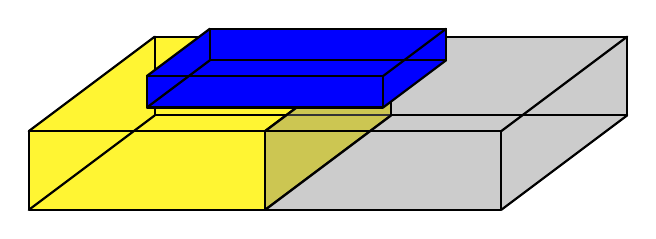
\begin{tikzpicture}[scale=2.0, line join=round, line cap=round]
      \def\s{3.0}
      \def\h{0.5}
      \def\w{1.5}

      \coordinate (I) at (0,-\h);
      \coordinate (J) at (\s - \w,-\h);
      \coordinate (K) at (\s - \w, -\h + \h);
      \coordinate (L) at (0,-\h + \h);
      \coordinate (M) at (0.8,0.6 -\h);
      \coordinate (N) at (\s+0.8 - \w,0.6 -\h);
      \coordinate (O) at (\s+0.8 - \w,0.6 -\h + \h);
      \coordinate (P) at (0.8,0.6 -\h + \h);
      % Fill faces (cube 2)
      \fill[yellow, opacity=0.8] (I)--(J)--(K)--(L)--cycle; % front
      \fill[yellow, opacity=0.8] (L)--(K)--(O)--(P)--cycle; % top
      \fill[yellow, opacity=0.8] (J)--(N)--(O)--(K)--cycle; % right side
      \draw[thick] (I)--(J)--(K)--(L)--cycle;
      \draw[thick] (M)--(N)--(O)--(P)--cycle;
      \draw[thick] (I)--(M) (J)--(N) (K)--(O) (L)--(P);

      \coordinate (I) at (\w, - \h);
      \coordinate (J) at (\s, - \h);
      \coordinate (K) at (\s, -0);
      \coordinate (L) at (\w, - 0);
      \coordinate (M) at (\w + 0.8,0.6 - \h);
      \coordinate (N) at (\s+0.8,0.6 - \h);
      \coordinate (O) at (\s+0.8,0.6 - \h + \h);
      \coordinate (P) at (\w + 0.8,0.6 - \h + \h);
      % Fill faces (cube 3)
      \fill[gray, opacity=0.4] (I)--(J)--(K)--(L)--cycle; % front
      \fill[gray, opacity=0.4] (L)--(K)--(O)--(P)--cycle; % top
      \fill[gray, opacity=0.4] (J)--(N)--(O)--(K)--cycle; % right side
      \draw[thick] (I)--(J)--(K)--(L)--cycle;
      \draw[thick] (M)--(N)--(O)--(P)--cycle;
      \draw[thick] (I)--(M) (J)--(N) (K)--(O) (L)--(P);

      % Define scale for blue cube
      \def\bluecubescale{0.5} % Adjust this value to make it smaller or larger
      \def\sblue{\s * \bluecubescale}
      \def\hblueactual{0.2} % Actual height of the blue cube, make it flatter
      \def\depthx_blue{0.8 * \bluecubescale} % Scaled x-shift for depth
      \def\depthyblue{0.6 * \bluecubescale} % Scaled y-shift for depth

      % Calculate horizontal offset to keep the blue cube centered on the base
      \pgfmathsetmacro\xoffsetblue{(\s - \sblue) / 2}

      % Calculate front-to-back offset to keep the blue cube centered on the base's top surface
      % The base's top surface depth in y-direction is 0.6 (without perspective shift)
      \pgfmathsetmacro\yoffsetbluedepth{(0.6 - \depthyblue) / 2}

      % Define coordinates for the blue cube, positioned on top of the base
      % The base's top front edge is at y=0
      \coordinate (A) at (\xoffsetblue, \yoffsetbluedepth);
      \coordinate (B) at (\xoffsetblue+\sblue, \yoffsetbluedepth);
      \coordinate (C) at (\xoffsetblue+\sblue, \yoffsetbluedepth + \hblueactual);
      \coordinate (D) at (\xoffsetblue, \yoffsetbluedepth + \hblueactual);
      % Back square (shifted) for perspective
      \coordinate (E) at (\xoffsetblue+\depthx_blue, \yoffsetbluedepth + \depthyblue);
      \coordinate (F) at (\xoffsetblue+\sblue+\depthx_blue, \yoffsetbluedepth + \depthyblue);
      \coordinate (G) at (\xoffsetblue+\sblue+\depthx_blue, \yoffsetbluedepth + \depthyblue + \hblueactual);
      \coordinate (H) at (\xoffsetblue+\depthx_blue, \yoffsetbluedepth + \depthyblue + \hblueactual);

      % Fill faces (cube 1) - now opaque
      \fill[blue] (A)--(B)--(C)--(D)--cycle; % front
      \fill[blue] (D)--(C)--(G)--(H)--cycle; % top
      \fill[blue] (B)--(F)--(G)--(C)--cycle; % right side
      % Draw faces and connecting edges
      \draw[thick] (A)--(B)--(C)--(D)--cycle;
      \draw[thick] (E)--(F)--(G)--(H)--cycle;
      \draw[thick] (A)--(E) (B)--(F) (C)--(G) (D)--(H);
    
    \end{tikzpicture}
    \caption{Illustration of the system: the blue is the material region~$\Omega_m$, the yellow and gray regions are dielectric materials:~$\Omega_1$ and~$\Omega_2$, respectively, non-filled regions are vacuum denoted as~$\Omega_0$.}
    \label{fig:system}
\end{figure*}


% \begin{figure}[htbp]
%     \centering
%     \begin{tikzpicture}[scale=1.0, line join=round, line cap=round]
%       \def\s{4.0}
%       \def\h{2.0}
%       \coordinate (A) at (0,0); \coordinate (B) at (\s,0);
%       \coordinate (C) at (\s,\h); \coordinate (D) at (0,\h);
%       \coordinate (E) at (\s, 0); \coordinate (F) at (2*\s, 0);
%       \coordinate (G) at (2*\s, \h); \coordinate (H) at (\s, \h);
%       \coordinate (I) at (0.5*\s, 1.5*\h); \coordinate (J) at (1.5*\s, 1.5*\h);
%       \coordinate (K) at (1.5*\s, \h); \coordinate (L) at (0.5*\s, \h);
%       \draw[thick] (A)--(B)--(C)--(D)--cycle;
%       \draw[thick] (E)--(F)--(G)--(H)--cycle;
%       \draw[thick] (I)--(J)--(K)--(L)--cycle;
%       \node at (1.3*\s, 1.3*\h) {$\Omega_m$};
%       \node at (\s/2, \h/2) {$\Omega_1$};
%       \node at (1.5*\s, \h/2) {$\Omega_2$};
%       \node at (2.2*\s, 1.2*\h) {$\Omega_0$};
%       \coordinate (S) at (0.8*\s, 1.25*\h);
%       \fill[gray, opacity=0.4] (S) circle (0.2*\h);
%       \node at (S) {$\rho(x)$};
%       \draw[->, thick] (\s/4,\h) -- (\s/4,\h+0.5) node[right,above] {$\V n$};
%       \draw[->, thick] (\s,\h/2) -- (\s-0.5,\h/2) node[midway,above] {$\V n$};
%       \draw[->, thick] (\s*3/4,\h) -- (\s*3/4,\h-0.5) node[right,below] {$\V n$};
%     \end{tikzpicture}
%     \caption{2D cartoon of the system geometry.  The gray blob is the
%       source density $\rho(x)$ supported in the material region $\Omega_m$;
%       $\Omega_{1,2}$ are dielectric slabs; the remainder is vacuum $\Omega_0$.
%       Arrows indicate the outward normal on each interface.}
%     \label{fig:system}
% \end{figure}

\section{Numerical Method}

In this section, we present the numerical method for solving the Poisson equation in Eq.~\eqref{eq:poisson} and evaluating the target integral accurately and efficiently.

\subsection{Overview}

To solve Eq.~\eqref{eq:poisson}, there are a few challenges that need to be addressed, which arise from the geometry of the system and physical properties of the solution.
% \begin{itemize}
%     \item[1.] The system includes multiple dielectric interfaces with sharp boundaries. 
%     \item [2.] The geometry of the system introduces edges and corners, where leads to singularities in the solution.
%     \item [3.] The aspect ratio of the system can be large, since we are trying to model layer materials.
%     \item [4.] Both source and target densities are continuous volume distributions and can overlap with the interfaces and each other.
% \end{itemize}

\paragraph{Sharp interfaces}
The first challenge is that the system includes multiple dielectric interfaces with sharp boundaries. 
Due to the sharp boundaries, directly discretizing the volume and solving the resulting linear system can be computationally expensive and may not achieve high accuracy due to the presence of singularities at the interfaces.
Instead, we will show that we first reformulate Eq.~\eqref{eq:poisson} as a boundary value problem defined on the union of the dielectric interfaces, which can be further transformed into a boundary integral equation (BIE) defined on the interfaces.

\paragraph{Edges and corners singularities}
The second challenge is that the geometry of the system introduces edges and corners, which leads to singularities in the solution.
After reformulating the problem as a BIE, we apply the Nystr\"om method to discretize it, where the unknown layer density is represented and integrated using tensor-product Gauss--Legendre nodes on each panel of the interface discretization.
However, for the edge and corner singularities, a uniform discretization of the interfaces is not sufficient to achieve high accuracy, and we need to apply an adaptive discretization strategy that refines the interface panels near the singularities and source-proximal regions.

\paragraph{Large aspect ratio}
The third challenge is that the aspect ratio of the system can be large, since we are modeling layered materials.
Then for each panel of the interface discretization, the standard quadrature may not be accurate enough for evaluating the layer potential at target points that are close to the panel, and we need to apply a near-field correction strategy to improve the accuracy of the layer potential evaluation in such cases.

\paragraph{Continuous volume densities}
The fourth challenge is that both source and target densities are continuous volume distributions that can be close to the interfaces and overlap with each other.
This is different from the classical BIE setting where the sources and targets are typically point charges or smooth functions supported away from the interfaces.
In this work, we develop a volume solver based on the truncated kernel method (TKM) to evaluate the incident potential generated by the source density, which serves as the right-hand side of the BIE, and also to evaluate the target integral once the layer potential is obtained.

\paragraph{Repeated Solves and Evaluations}
In practice, we need to evaluate the four-indices integrals for a large number of source and target densities, which requires repeated solves of the Poisson equation and evaluations of the target integral.
For the same source with different targets, we use a post-refinement strategy to reuse the result.

In the following sections, we will show how to resolve those challenges one by one, and present the details of the numerical method for solving the Poisson equation and evaluating the target integral.

\subsection{The Boundary Integral Formulation}\label{sec:bie}

We first show that Eq.~\eqref{eq:poisson} can be reformulated as a boundary-value problem (BVP) for the potential $\phi$ in the piecewise constant dielectric medium:
\begin{equation}\label{eq:bvp}
    \begin{cases}
        \epsilon_m \Delta_x \phi(x) = -\rho(x), & x \in \Omega_m,\\
        \Delta_x \phi(x) = 0, & x \notin \Omega_m,\\
        \phi\mid_{\partial \Omega_i} = \phi\mid_{\partial \Omega_j}, &
            x \in \partial\Omega_i \cap \partial\Omega_j,\\
        \epsilon_i \partial_{\V n} \phi\mid_{\partial \Omega_i}
            = \epsilon_j \partial_{\V n} \phi\mid_{\partial \Omega_j}, &
            x \in \partial\Omega_i \cap \partial\Omega_j,\\
        \phi(x) \to 0, & \abs{x} \to \infty.
    \end{cases}
\end{equation}
The first two lines are the Poisson equation in the material region and the Laplace equation in the vacuum and other dielectric regions, respectively.
The third and fourth lines are the interfacial continuity and flux-matching conditions, where $\partial\Omega_i$ denotes the boundary of the region $\Omega_i$, and $\partial_{\V n}$ denotes the normal derivative with respect to the outward normal $\V n$ of the region.
The last line is the condition at infinity, which ensures the uniqueness of the solution.

However, Eq.~\ref{eq:bvp} is still a partial differential equation defined in the volume, and we need to reformulate it as a boundary integral equation defined on the interfaces to take advantage of the piecewise constant nature of the permittivity and the fact that the sources and targets are supported in the volume.
To achieve this, we first split the potential as two parts,
\begin{equation}
    \phi(x) = u_{\text{inc}}(x) + u(x).
\end{equation}
$u_{\text{inc}}$ is the incident potential generated by the source density $\rho$ in free space:
\begin{equation}
    u_{\text{inc}}(x) = \frac{1}{4\pi\epsilon_m}
        \int \frac{\rho(x')}{\abs{x-x'}}\, \mathrm{d}x'.
\end{equation}
The incident potential naturally satisfies the following conditions:
\begin{equation}
    \begin{cases}
        \epsilon_m \Delta_x u_{\text{inc}}(x) = -\rho(x), & x \in \Omega_m,\\
        \Delta_x u_{\text{inc}}(x) = 0, & x \notin \Omega_m,\\
        u_{\text{inc}}\mid_{\partial \Omega_i} = u_{\text{inc}}\mid_{\partial \Omega_j}, &
            x \in \partial\Omega_i \cap \partial\Omega_j,\\
        \partial_{\V n} u_{\text{inc}}\mid_{\partial \Omega_i}
            = \partial_{\V n} u_{\text{inc}}\mid_{\partial \Omega_j}, &
            x \in \partial\Omega_i \cap \partial\Omega_j,\\
        u_{\text{inc}}(x) \to 0, & \abs{x} \to \infty.
    \end{cases}
\end{equation}
Then for the scattered potential $u$, we make use of the single layer potential representation, which is a standard approach for solving the Laplace equation in the presence of interfaces:
\begin{equation}
    u(x) = \frac{1}{4\pi}\int_\Gamma \frac{\sigma(x')}{\abs{x-x'}}\, \mathrm{d}S(x'),
\end{equation}
where $\Gamma$ denotes the union of dielectric interfaces, and $\sigma$ is the single layer density defined on $\Gamma$ that needs to be solved for.
The scattered potential $u$ automatically satisfies the following conditions:
\begin{equation}
    \begin{cases}
        \Delta_x u(x) = 0, & x \in \Omega_*,\\
        u\mid_{\partial \Omega_i} = u\mid_{\partial \Omega_j}, &
            x \in \partial\Omega_i \cap \partial\Omega_j,\\
        u(x) \to 0, & \abs{x} \to \infty.
    \end{cases}
\end{equation}
Thus, the remaining conditions that need to be satisfied are the flux-matching conditions at the interfaces, which can be written as
\begin{equation}\label{eq:flux_matching}
    \epsilon_i \partial_{\V n} u\mid_{\partial \Omega_i} + \epsilon_i \partial_{\V n} u_{\text{inc}}\mid_{\partial \Omega_i}
        = \epsilon_j \partial_{\V n} u_{\text{inc}}\mid_{\partial \Omega_j} + \epsilon_j \partial_{\V n} u\mid_{\partial \Omega_j}, 
            \quad x \in \partial\Omega_i \cap \partial\Omega_j.
\end{equation}
Using the standard jump relation for the single layer potential,
\begin{equation}
    \partial_{\V n} u(x) \mid_{\pm} = \left(\pm \frac{1}{2}I + D^T\right)\sigma(x), \qquad x \in \Gamma,
\end{equation}
where~$\pm$ denotes the limit from the respective sides of the interface and $D^T$ is the adjoint of the double layer operator defined as
\begin{equation}
    D^T \sigma(x) = \frac{1}{4\pi}\int_\Gamma \frac{(x-x')\cdot \V n(x)}{\abs{x-x'}^3}\sigma(x')\, \mathrm{d}S(x'),
\end{equation}
the interfacial flux-matching condition in Eq.~\eqref{eq:flux_matching} reduces to the Fredholm integral equation of the second kind~\cite{greengard1994numerical}
\begin{equation}\label{eq:sl}
    \frac{1}{2}\gamma(x)^{-1} \sigma(x) + D^T \sigma(x) = -\partial_{\V n} u_{\text{inc}}(x), \qquad x \in \Gamma,
\end{equation}
where~$\gamma$ is the dielectric contrast defined as
\begin{equation}
    \gamma(x) = \frac{\epsilon_i - \epsilon_j}{\epsilon_i + \epsilon_j}, \qquad x \in \partial\Omega_i \cap \partial\Omega_j, 
\end{equation}
a piecewise constant function defined on the interfaces that depends on the permittivity of the adjacent regions.
For simplicity, we write Eq.~\eqref{eq:sl} as 
\begin{equation}
    A \sigma = f\;.
\end{equation}

\subsection{Nystr\"om discretization and adaptive quadrature}\label{sec:quadrature}

We now discretize the second-kind boundary integral equation in Eq.~\eqref{eq:sl} on a panelized representation of the interface~$\Gamma$.
We write
\begin{equation}
\Gamma = \bigcup_{m=1}^{M} P_m,
\end{equation}
where each $P_m$ is a flat rectangular panel equipped with a local affine parametrization
\begin{equation}
\mathbf X_m:[-1,1]^2 \to P_m.
\end{equation}
On each panel, we place a tensor-product Gauss--Legendre rule of order $p$ in the two local parametric directions.
If $\{\xi_a,\omega_a\}_{a=1}^p$ and $\{\eta_b,\omega_b\}_{b=1}^p$ denote the one-dimensional Gauss--Legendre nodes and weights, then the corresponding physical quadrature nodes are
\begin{equation}
x_{mab} = \mathbf X_m(\xi_a,\eta_b),
\end{equation}
with surface weights
\begin{equation}
w_{mab} = J_m(\xi_a,\eta_b)\,\omega_a\omega_b,
\end{equation}
where $J_m$ is the Jacobian of the panel parametrization.

Let $\{x_i,w_i,\V{n}_i\}_{i=1}^N$ denote the collection of all quadrature nodes, weights, and outward normals over all panels, and define
\begin{equation}
\sigma_i = \sigma(x_i), \qquad
f_i = -\partial_{\V n}u_{\mathrm{inc}}(x_i).
\end{equation}
Collocating Eq.~\eqref{eq:sl} at each quadrature node $x_i$ and approximating the surface integral by panelwise tensor-product Gauss--Legendre quadrature gives the Nystr\"om discretization
\begin{equation}\label{eq:nystrom_discrete}
    \frac{1}{2}\gamma(x_i)^{-1}\sigma_i
    +
    \sum_{\substack{j=1 \\ j\neq i}}^{N}
    \frac{(x_i-x_j)\cdot \V{n}_i}{4\pi |x_i-x_j|^3}\,
    \sigma_j\,w_j
    =
    f_i,
    \qquad i=1,\dots,N.
\end{equation}
Collecting all nodal values into the vectors
\begin{equation}
\V{\sigma} = (\sigma_1,\dots,\sigma_N)^\top,
\qquad
\V{f} = (f_1,\dots,f_N)^\top,
\end{equation}
we obtain the linear system
\begin{equation}\label{eq:linsys}
    \M{A}\V{\sigma} = \V{f},
\end{equation}
with matrix entries
\begin{equation}
    A_{ij} =
    \begin{cases}
        \displaystyle \frac{1}{2}\gamma(x_i)^{-1}, & i=j,\\[6pt]
        \displaystyle \frac{(x_i-x_j)\cdot \V{n}_i}{4\pi |x_i-x_j|^3}\,w_j, & i\neq j.
    \end{cases}
\end{equation}
This discretization preserves the second-kind structure of the continuous integral equation and yields high-order accuracy on interface patches that are sufficiently smooth and well resolved.

% In the part, describe the adaptive refinement
A uniform panelization is, however, inadequate for the dielectric configurations considered here.
First, the right-hand side~$f$ of Eq.~\eqref{eq:sl} can vary rapidly when the sources are close to the interface, and so do the layer density $\sigma$.
A fix panel size is not sufficient to resolve both of them accurately.
Second, the layer density $\sigma$ itself develops integrable singularities near edges and corners of the dielectric interfaces, which can not be resolved by a uniform panelization.
To address these issues, we apply an adaptive panel refinement strategy that refines the panels near edges and corners of the interfaces, as well as near the source-proximal regions where the right-hand side varies rapidly.

In our model, we assume that all dielectric interfaces are composed of flat rectangular panels, which is a reasonable approximation for bulk and layered materials.
Instead of increasing the quadrature order uniformly, we fix the order as~$p$, and employ a \emph{dyadic} refinement strategy, in which each panel is subdivided into four child panels recursively until a prescribed criterion is satisfied.

The first part of the refinement criterion is RHS-driven.
With a given tolerance~$\varepsilon$, the refinement criterion is based on the local interpolation error of the right-hand side $f$ on each panel, which is computed by comparing $f$ with a polynomial interpolant of degree $p-1$ in each local parametric direction.
To make this more precise, let $P \subset \Gamma$ be a panel, and let $(\xi,\eta)\in[-1,1]^2$ denote its local parametric coordinates.
On each panel, the restriction of the right-hand side is approximated by a tensor-product polynomial interpolant
\begin{equation}
g_P \in \mathbb{Q}_{p-1,p-1}([-1,1]^2) = \mathbb{P}_{p-1}([-1,1]) \otimes \mathbb{P}_{p-1}([-1,1]),
\end{equation}
where $\mathbb{Q}_{p-1,p-1}([-1,1]^2)$ denotes the space of polynomials of degree at most $p-1$ in each local parametric direction.
We then monitor the local interpolation error and refine the panel until 
\begin{equation}\label{eq:refine_criterion}
    \norm{g_P - f}_{L^2(P)} < \varepsilon.
\end{equation}

Then the second part of the refinement criterion is geometry-driven.
For each panel that is adjacent to an edge or corner of the interface, we refine it until the panel size is smaller than a prescribed threshold~$\delta$.
Although it can not really solve the singularity of~$\sigma$, but it can lead to a geometric convergence, as will be shown in the numerical results, which is sufficient for our particular application.


\begin{figure}[htbp]
    \centering

    \subfloat[]{%
        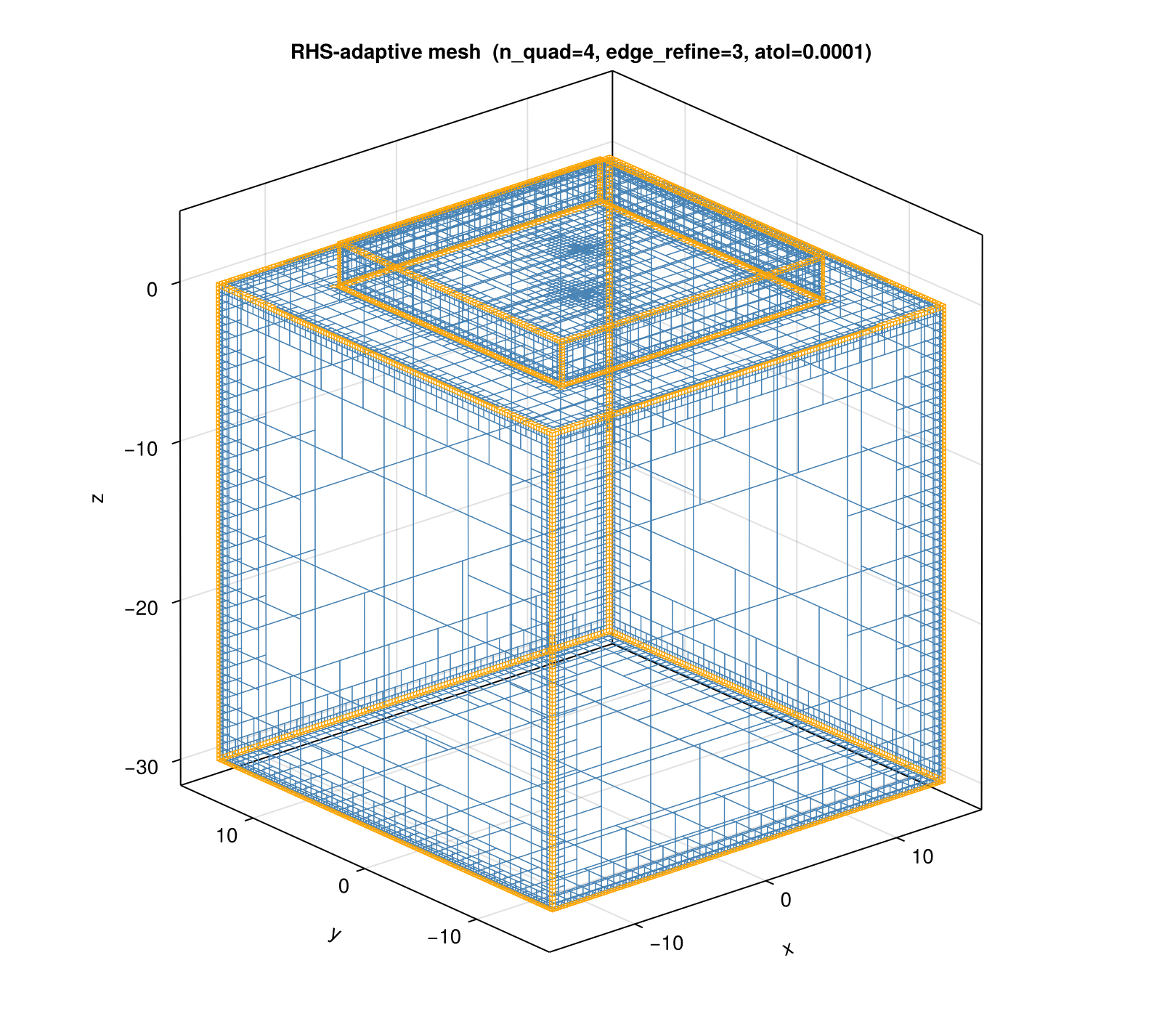
\includegraphics[width=0.48\textwidth,height=0.28\textheight,keepaspectratio]{figs/refined_boxes.png}%
    }
    \hfill
    \subfloat[]{%
        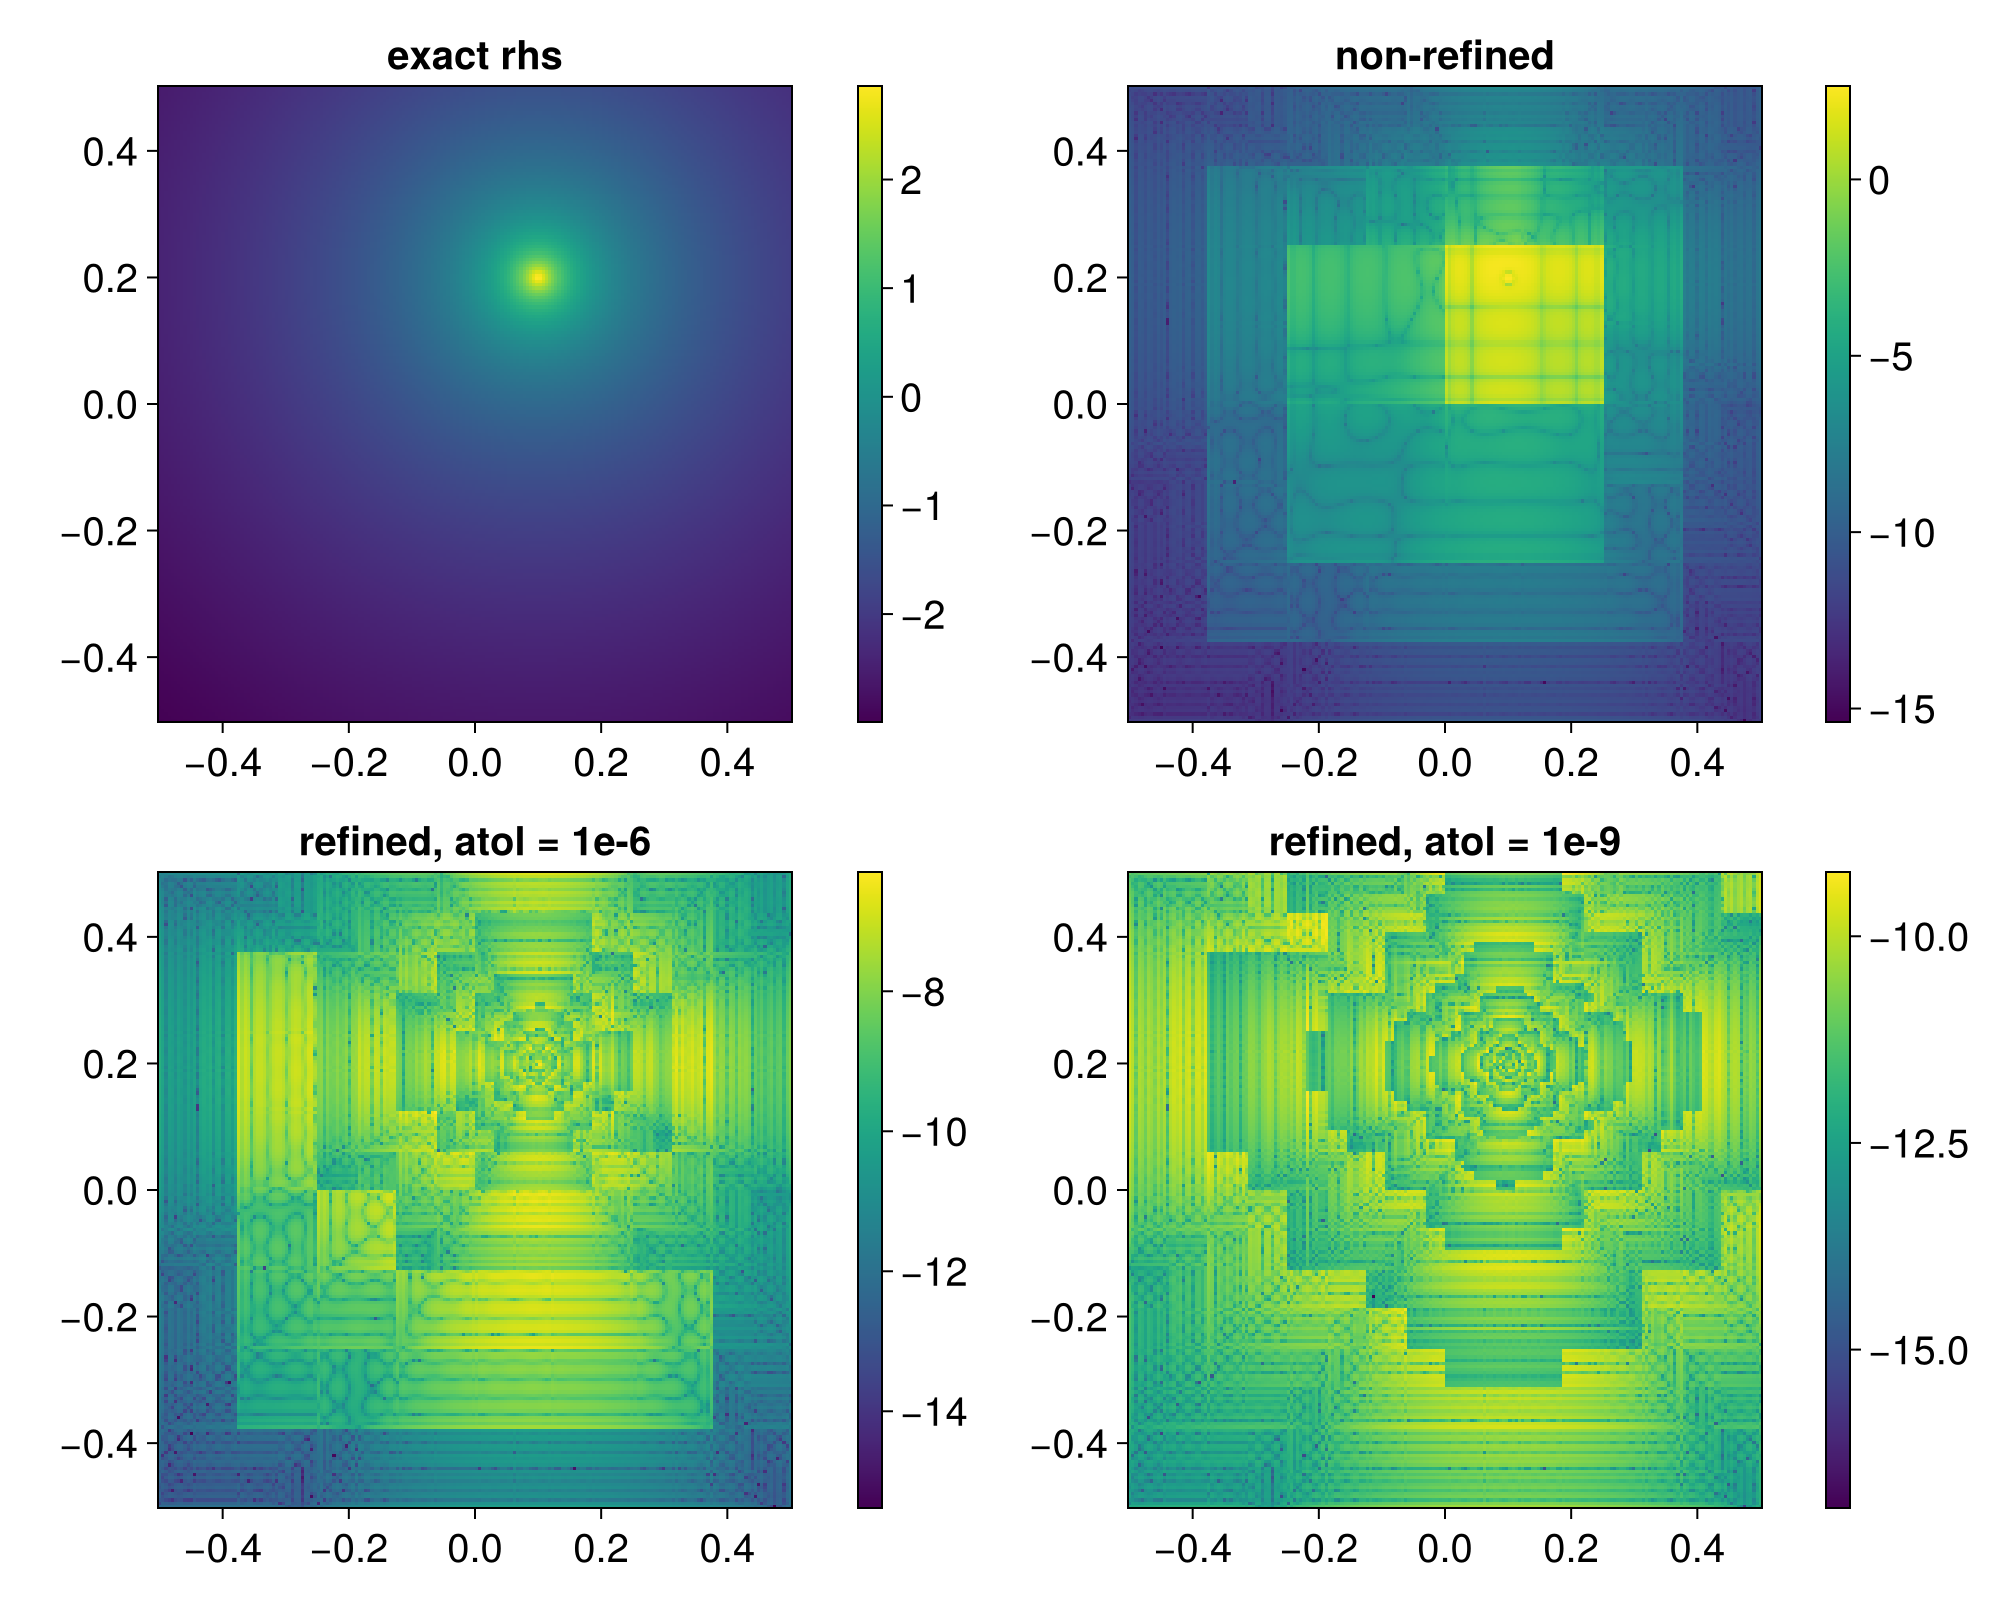
\includegraphics[width=0.48\textwidth,height=0.28\textheight,keepaspectratio]{../codes/box3d_corrected/figs/rhs_solve_refined_d_0.01.png}%
    }
    
    \caption{Illustration of the adaptive discretization for the right-hand side of the BIE in Eq.~\eqref{eq:sl} for a point source close to the interface $\Gamma$: left, the adaptive dyadic refinement of the interface panels; right, the value and error of the polynomial interpolant of the right-hand side.}
    \label{fig:rhs}
\end{figure}

An example is shown in Fig.~\ref{fig:rhs}. 
In Fig.~\ref{fig:rhs}(a), we show the adaptive dyadic refinement of the interface panels, which is more refined near the source and the edges of the interface (shown in orange).
In Fig.~\ref{fig:rhs}(b), we plot the absolute interpolation error in the right-hand side of the BIE for a point source located close to the interface~$\Gamma$.

\subsection{Near-field evaluation of layer potentials}\label{sec:nearfield}

After the adaptive panel refinement has been applied, both the geometry and the layer density~$\sigma$ are well resolved on the underlying Nystr\"om grid.
Luckily, we only evaluate the adjoint double-layer potential, which has no contribution to other points on the same flat surface.
However, the standard panelwise quadrature evaluation may still fail to achieve high accuracy when the target point is close to the source panel.
Such situations are common when assembling or applying the discrete operator~$\M{A}$ for layered materials with large aspect ratios, where large interface panels can remain geometrically close to one another.
In such cases, the quadrature error is no longer controlled effectively by the nominal order $p$ alone, and additional local resolution is required at the evaluation stage.
At the same time, it is undesirable to refine or upsample the underlying panel discretization globally, since this would increase the number of degrees of freedom and the cost of solving the BIE.
In this section, we describe a simple near-field evaluation method.

To detect this regime, we use a simple distance-based criterion tied to the local tensor-product Gauss--Legendre grid.
For each panel $P$, let $h_P$ denote the smallest local grid spacing on $P$, namely the minimum distance between neighboring Gauss--Legendre nodes after mapping to the physical panel.
More precisely, we define
\begin{equation}
    h_P = \min \left(\frac{L_\xi}{p}, \frac{L_\eta}{p} \right),
\end{equation}
where $L_\xi$ and $L_\eta$ are the side lengths of the physical panel in the two local parametric directions,
so that the near-field criterion depends not only on the panel geometry but also on the local quadrature resolution.
We classify the interaction between a target point $x$ and a panel $P$ as a near interaction whenever
\begin{equation}
    d(x,P) \le 5 h_P,
\end{equation}
where $d(x,P)$ denotes the Euclidean distance from $x$ to the panel $P$. 
In other words, we apply a $5h$ rule~\cite{barnett2014evaluation}: whenever the target lies within five local Gauss--Legendre grid spacings of a panel, the interaction is treated as near-field.

For each target--panel pair $(x,P)$ satisfying the $5h$ criterion, we replace the standard quadrature evaluation by a corrected local operator constructed through upsampling. 
Let $\sigma_P$ denote the restriction of the layer density to the source panel $P$, represented on the original tensor-product Gauss--Legendre grid. 
We then lift $\sigma_P$ to a finer tensor-product grid on the same panel and use this refined representation to assemble a corrected interaction matrix, denoted by $A^{\mathrm{near}}_{x,P}$. 
The contribution of the panel $P$ to the layer potential at the target $x$ is then approximated by
\begin{equation}\label{eq:nearfield_upsample}
    u_P(x) \approx A^{\mathrm{near}}_{x,P}\,\sigma_P.
\end{equation}
By contrast, for source--target pairs outside the near-field regime, we retain the standard Nystr\"om evaluation
\begin{equation}
    u_P(x) \approx A^{\mathrm{std}}_{x,P}\,\sigma_P,
\end{equation}
where $A^{\mathrm{std}}_{x,P}$ denotes the row block associated with the original tensor-product Gauss--Legendre quadrature on $P$.

For target points that coincide with Nystr\"om collocation nodes, these corrected panelwise evaluations induce a sparse correction to the discrete adjoint double-layer operator.
More precisely, if $x_i$ is a target node and $P$ is a source panel in its near field, we define the corrected row block by
\begin{equation}
    A^{\mathrm{corr}}_{x_i,P} = A^{\mathrm{near}}_{x_i,P} - A^{\mathrm{std}}_{x_i,P}.
\end{equation}
Only near target--panel pairs contribute nonzero blocks, so collecting all such corrections produces a sparse matrix, denoted by $D^T_{\mathrm{corr}}$.
Accordingly, the discrete BIE is applied in the form
\begin{equation}\label{eq:nearfield_corrected_A}
    \M{A} = \frac{1}{2}\M{\Gamma}^{-1} + D^T + D^T_{\mathrm{corr}},
\end{equation}
where $D^T$ is the standard Nystr\"om matrix assembled from the uncorrected panelwise quadrature, and $D^T_{\mathrm{corr}}$ replaces those row blocks for which the $5h$ criterion is triggered.

% \begin{figure}[htbp]
%     \centering
%     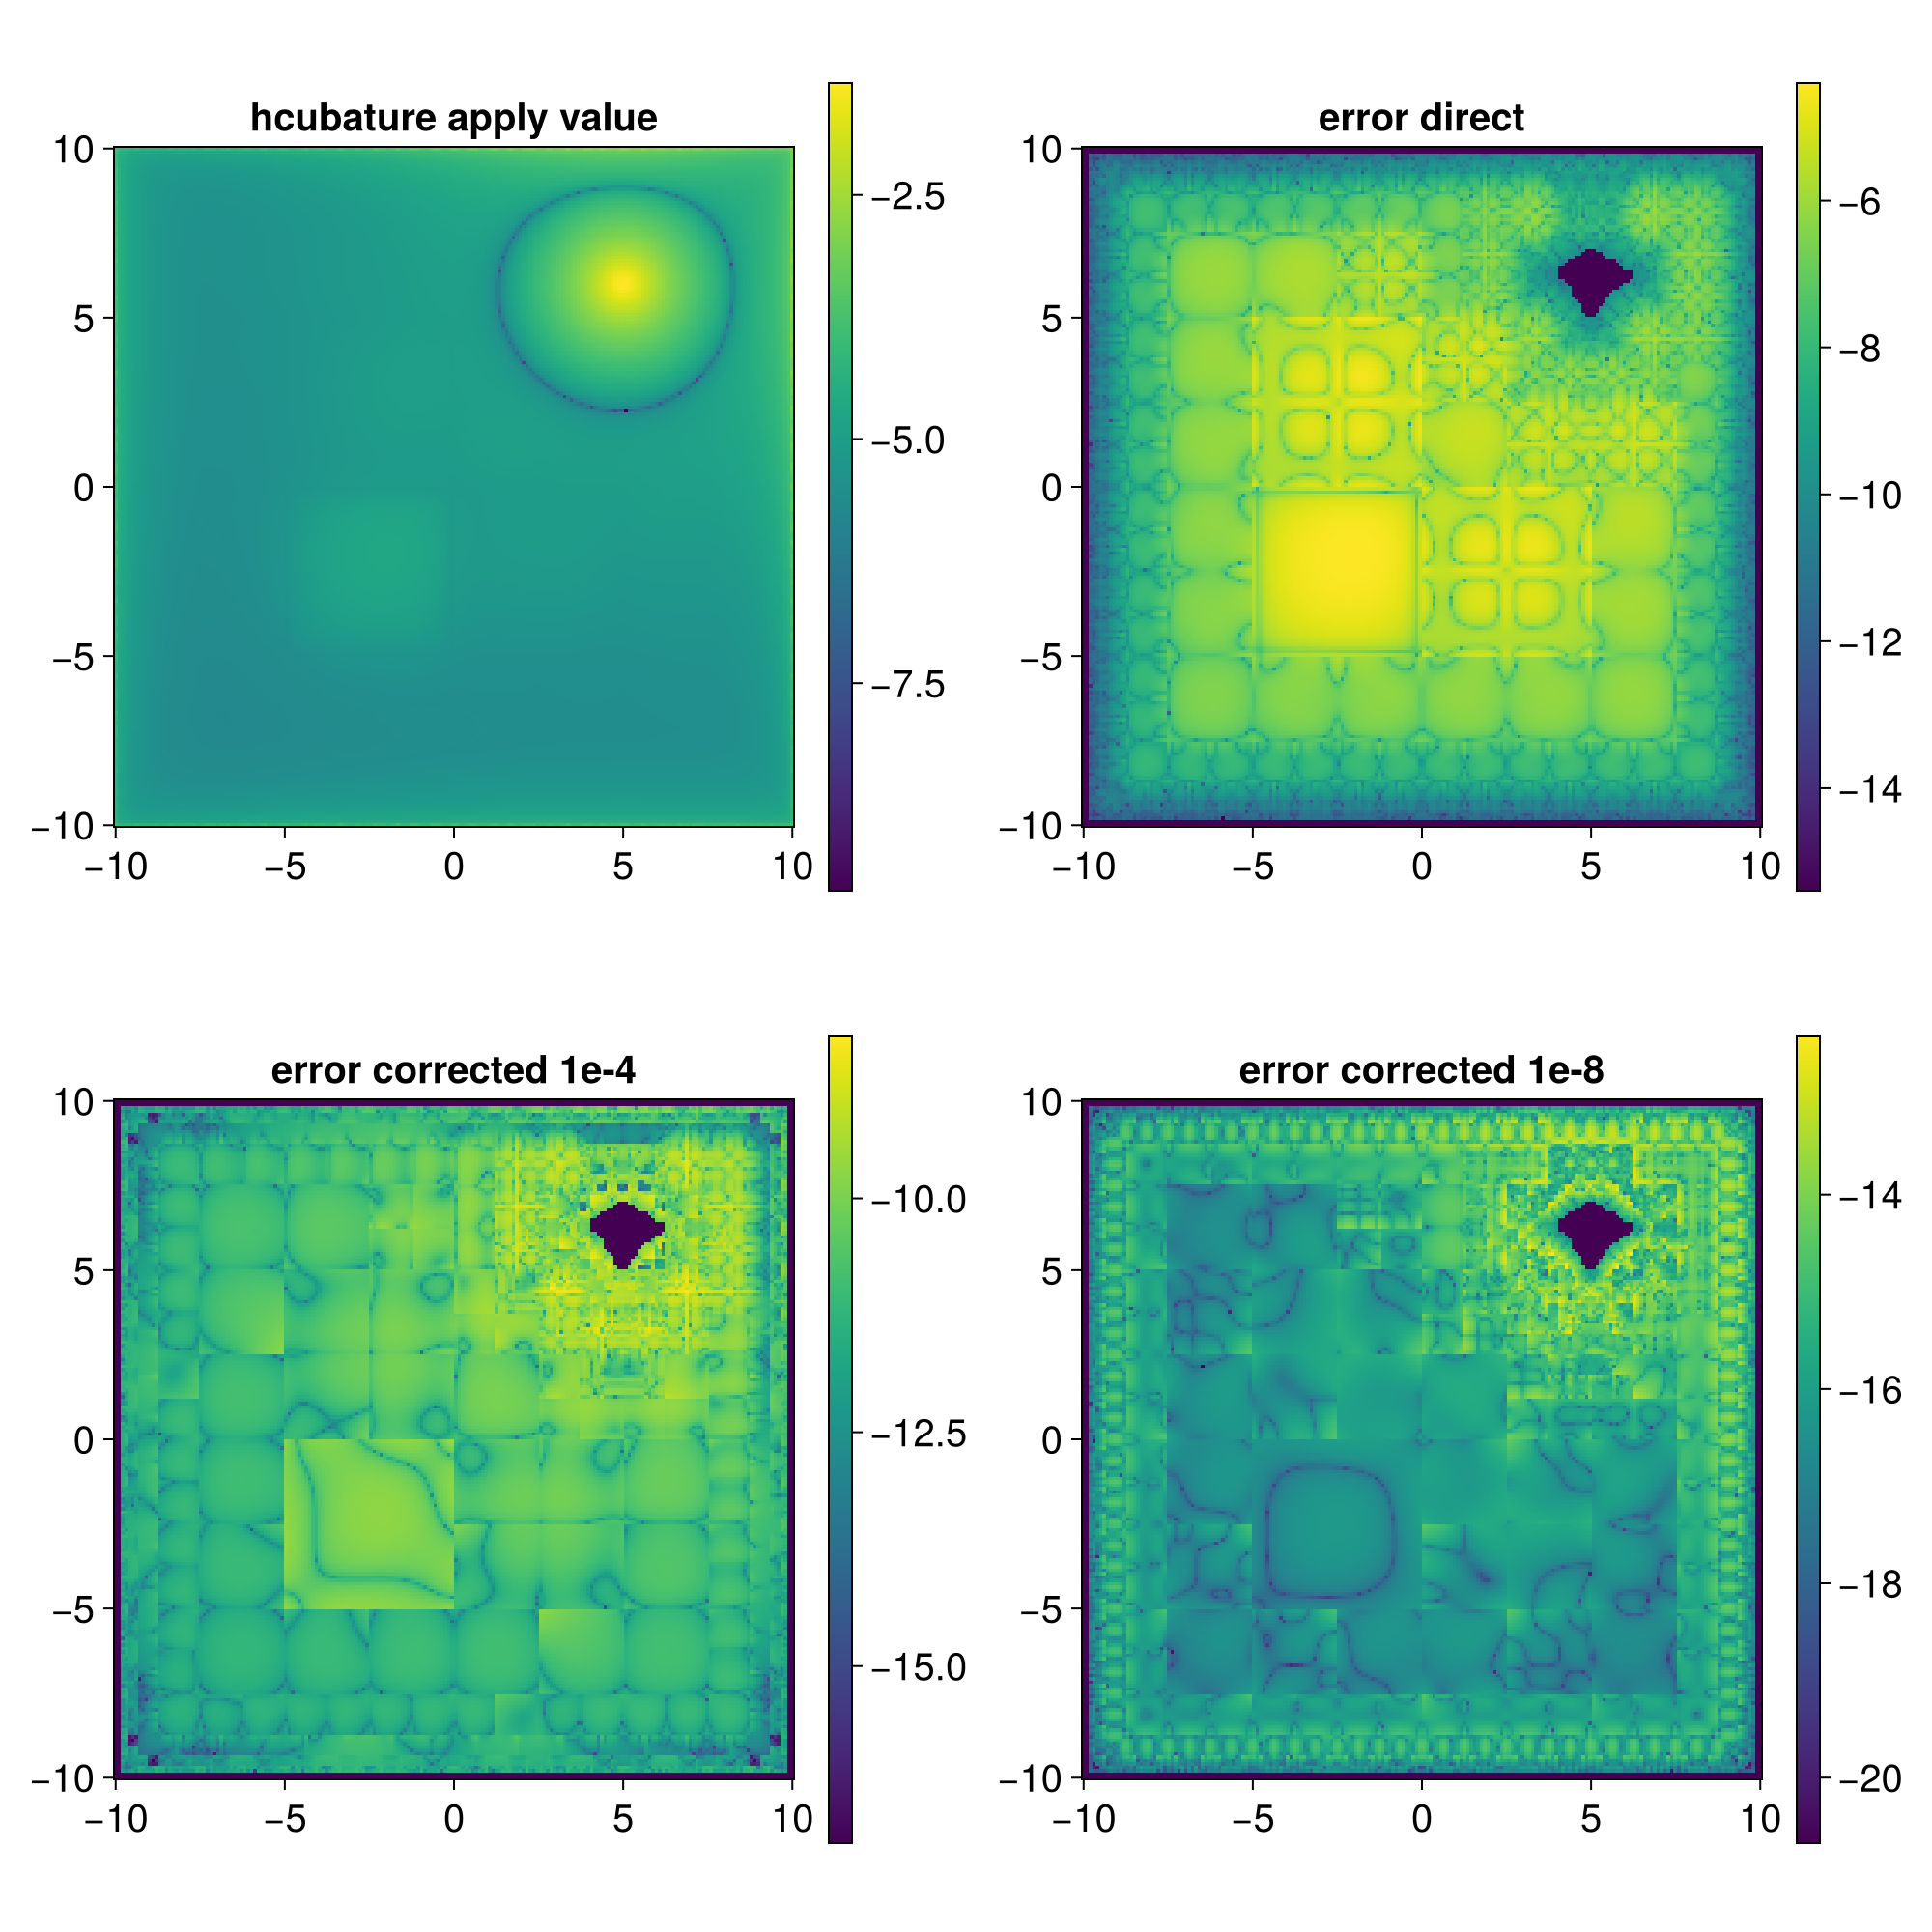
\includegraphics[width=0.8\textwidth]{../codes/box3d_corrected/figs/near_correction_near_source.png}
%     \caption{Illustration of the near-field evaluation of the layer potential for a target point $x$ close to a panel $P$. The near-field correction is applied whenever the distance from $x$ to $P$ is less than five local grid spacings $h_P$.}
%     \label{fig:near_field}
% \end{figure}

The role of this near-field treatment is complementary to that of dyadic panel refinement. 
The panel refinement controls the representation error by resolving geometric singularities and localized variation in the density. 
The near-field correction, on the other hand, controls the evaluation error for geometrically close source--target pairs, while leaving the underlying Nystr\"om degrees of freedom unchanged. 
Accordingly, the correction is invoked only when the $5h$ criterion is satisfied.
An example of the neighbor panels that are subject to the near-field correction for a given source panel is shown in Fig.~\ref{fig:near_field}.

\begin{figure}[htbp]
    \centering
    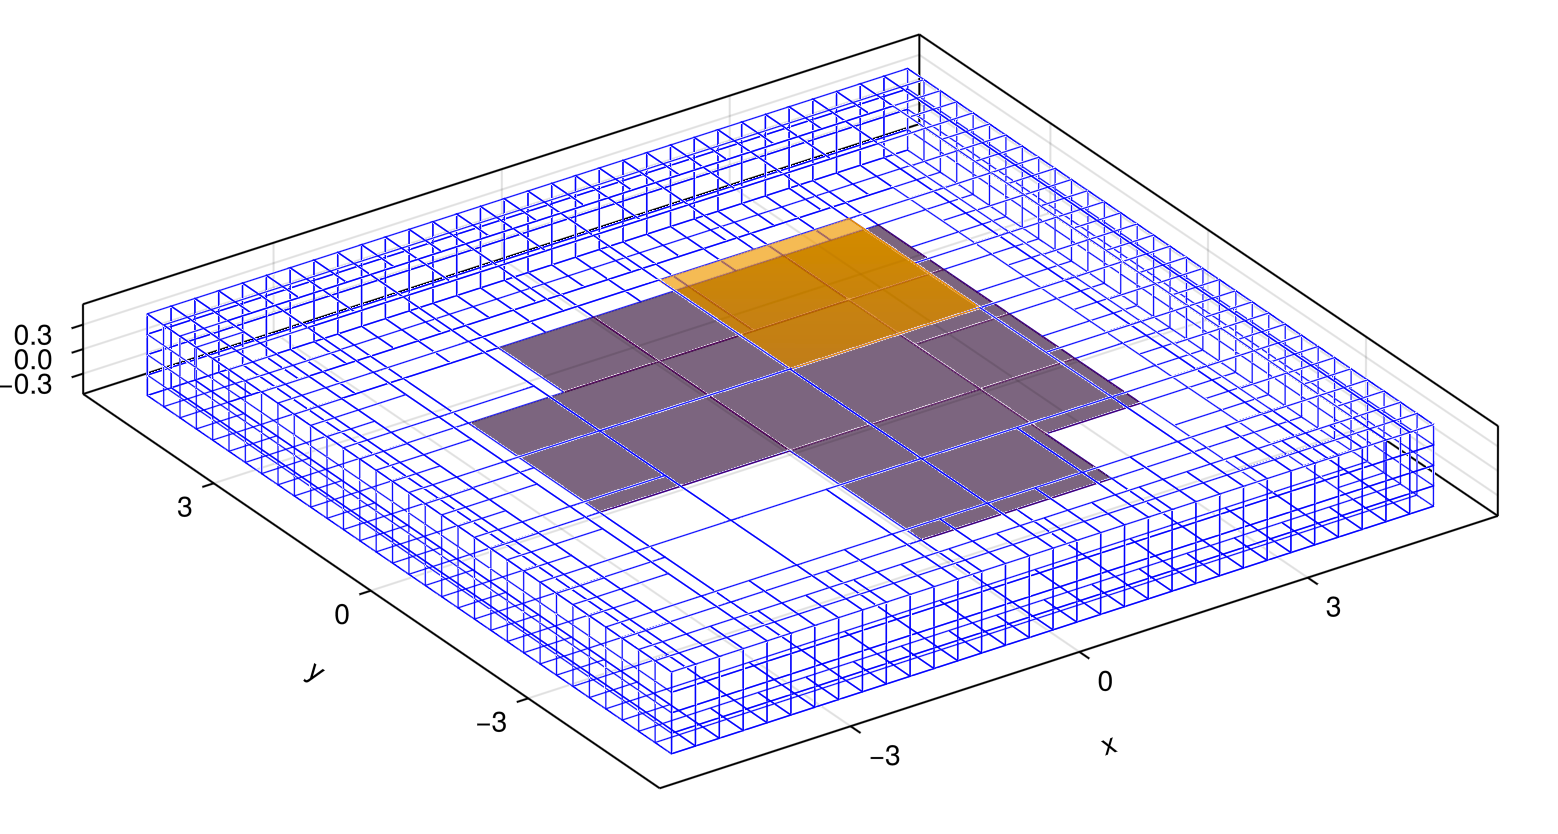
\includegraphics[width=0.8\textwidth]{figs/highlight_neighbors_demo.png}
    \caption{Illustraction of the neighbor panels (in purple) of a source panel (in orange) that are needed for the near-field correction. The aspect ration of the system is 10.}
    \label{fig:near_field}
    
\end{figure}

\begin{remark}
    The 5$h$ rule is a heuristic that has been found to be effective for about 6 to 8 digits of accuracy in practice. For higher accuracy, a factor larger than 5, such as 8, may be needed.
\end{remark}

\subsection{TKM volume solver for the incident potential}\label{sec:tkm}

In this section, we describe our strategy for evaluating the incident potential $u_{\mathrm{inc}}$ generated by the source density $\rho$, which serves as the right-hand side of the BIE in Eq.~\eqref{eq:sl}, as well as for evaluating the target integral once the layer potential is obtained.
However, this integral can be near-singular or even singular when the target point is close to or inside the source region, and it can be expensive to evaluate by direct quadrature in such cases.
Thus, we apply a Fourier-based volume solver based on the truncated kernel method (TKM) to evaluate this integral efficiently and accurately in the near field.

We assume that the source density \(\rho\) is a smooth function supported entirely in a single material region \(\Omega_m\), and that it is represented on a local uniform Cartesian grid. 
Under this assumption, the incident potential
\begin{equation}
    u_{\mathrm{inc}}(x)
    =
    \frac{1}{4\pi \epsilon_m}
    \int_{\Omega_m}
    \frac{\rho(y)}{|x-y|}
    \,dy
\end{equation}
is naturally evaluated by a Fourier-based volume solver.

To this end, we use a truncated kernel method~\cite{VICO2016191} (TKM) for the three-dimensional Poisson equation. 
Let
\begin{equation}
    G(x)=\frac{1}{4\pi |x|}
\end{equation}
be the free-space Green's function, and define the truncated kernel
\begin{equation}
    G_L(x)
    =
    \begin{cases}
        G(x), & |x|<L,\\
        0, & |x|\ge L.
    \end{cases}
\end{equation}
If the source support and the target region are contained in a rectangular box of side lengths \((l_x,l_y,l_z)\), then choosing
\begin{equation}
    L=\sqrt{l_x^2+l_y^2+l_z^2}
\end{equation}
ensures that \(G_L(x-y)=G(x-y)\) throughout the interaction region. 
Hence
\begin{equation}
    u_{\mathrm{inc}}(x)
    =
    \frac{1}{\epsilon_m}
    \int_{\mathbb{R}^3} G_L(x-y)\rho(y)\,dy.
\end{equation}

The Fourier transform of \(G_L\) is explicit,
\begin{equation}
    \widehat{G}_L(k)
    =
    2\left(\frac{\sin(L|k|/2)}{|k|}\right)^2,
\end{equation}
so that
\begin{equation}\label{eq:tkm_convolution}
    u_{\mathrm{inc}}(x)
    =
    \frac{1}{(2\pi)^3\epsilon_m}
    \int_{\mathbb{R}^3}
    \widehat{G}_L(k)\,\widehat{\rho}(k)\,e^{ik\cdot x}\,dk.
\end{equation}
Since \(\rho\) is sampled on a uniform grid and is assumed smooth, this convolution can be evaluated efficiently by FFT on a truncated Fourier domain.

To evaluate the Fourier integral numerically, we replace it by a trapezoidal sum on a uniform grid in \(k\)-space. 
If \(\Delta k_x,\Delta k_y,\Delta k_z\) denote the Fourier mesh spacings, then the associated real-space periods are
\begin{equation}
    P_x=\frac{2\pi}{\Delta k_x},\qquad
    P_y=\frac{2\pi}{\Delta k_y},\qquad
    P_z=\frac{2\pi}{\Delta k_z}.
\end{equation}
A sufficient condition for avoiding aliasing from the periodic images of the truncated kernel is
\begin{equation}
    P_x \ge l_x + L,\qquad
    P_y \ge l_y + L,\qquad
    P_z \ge l_z + L,
\end{equation}
or equivalently
\begin{equation}
    \Delta k_x \le \frac{2\pi}{l_x+L},\qquad
    \Delta k_y \le \frac{2\pi}{l_y+L},\qquad
    \Delta k_z \le \frac{2\pi}{l_z+L}.
\end{equation}
Thus, the Fourier grid must be fine enough that the periodized copies of the truncated convolution remain outside the physical domain of interaction. 
On the other hand, if \(\rho\) is represented on a uniform physical grid with spacing \(\Delta x\), then its discrete Fourier transform has Nyquist wavenumber
\begin{equation}
    k_{\mathrm{Nyq}}=\frac{\pi}{\Delta x},
\end{equation}
and the Fourier cutoff \(k_{\max}\) must satisfy
\begin{equation}
    k_{\max}<k_{\mathrm{Nyq}}.
\end{equation}
In practice, \(k_{\max}\) is chosen so that \(|\widehat{\rho}(k)|\) is already below the target tolerance near \(k_{\max}\); since \(\rho\) is assumed smooth, this can be achieved with a moderate Fourier bandwidth. 

The TKM solver is used only in the near field. 
When evaluating the right-hand side of the boundary-integral equation or the associated volume integrals, we apply the same \(5h\) criterion as in the near evaluation of layer potentials. 
If a target lies within \(5h\) of the source region, the corresponding contribution is evaluated by the TKM volume solver; otherwise it is treated by the FMM-based far-field solver. 
% In particular, \(u_{\mathrm{inc}}\) and \(\partial_{\V n}u_{\mathrm{inc}}\) on the dielectric interfaces provide the right-hand side
% \begin{equation}
%     \frac{1}{2}\frac{\epsilon_i+\epsilon_j}{\epsilon_i-\epsilon_j}\sigma(x)
%     + D^T\sigma(x)
%     =
%     -\partial_{\V n}u_{\mathrm{inc}}(x),
% \end{equation}
% thereby coupling the Fourier-based near-field volume solve to the sharp-interface boundary-integral formulation.
An example of the accuracy of the TKM volume solver for the incident potential \(u_{\mathrm{inc}}\) is shown in Fig.~\ref{fig:tkm}, where we plot the error of \(u_{\mathrm{inc}}\) against direct summation with the sampling points.

\begin{figure}[htbp]
    \centering
    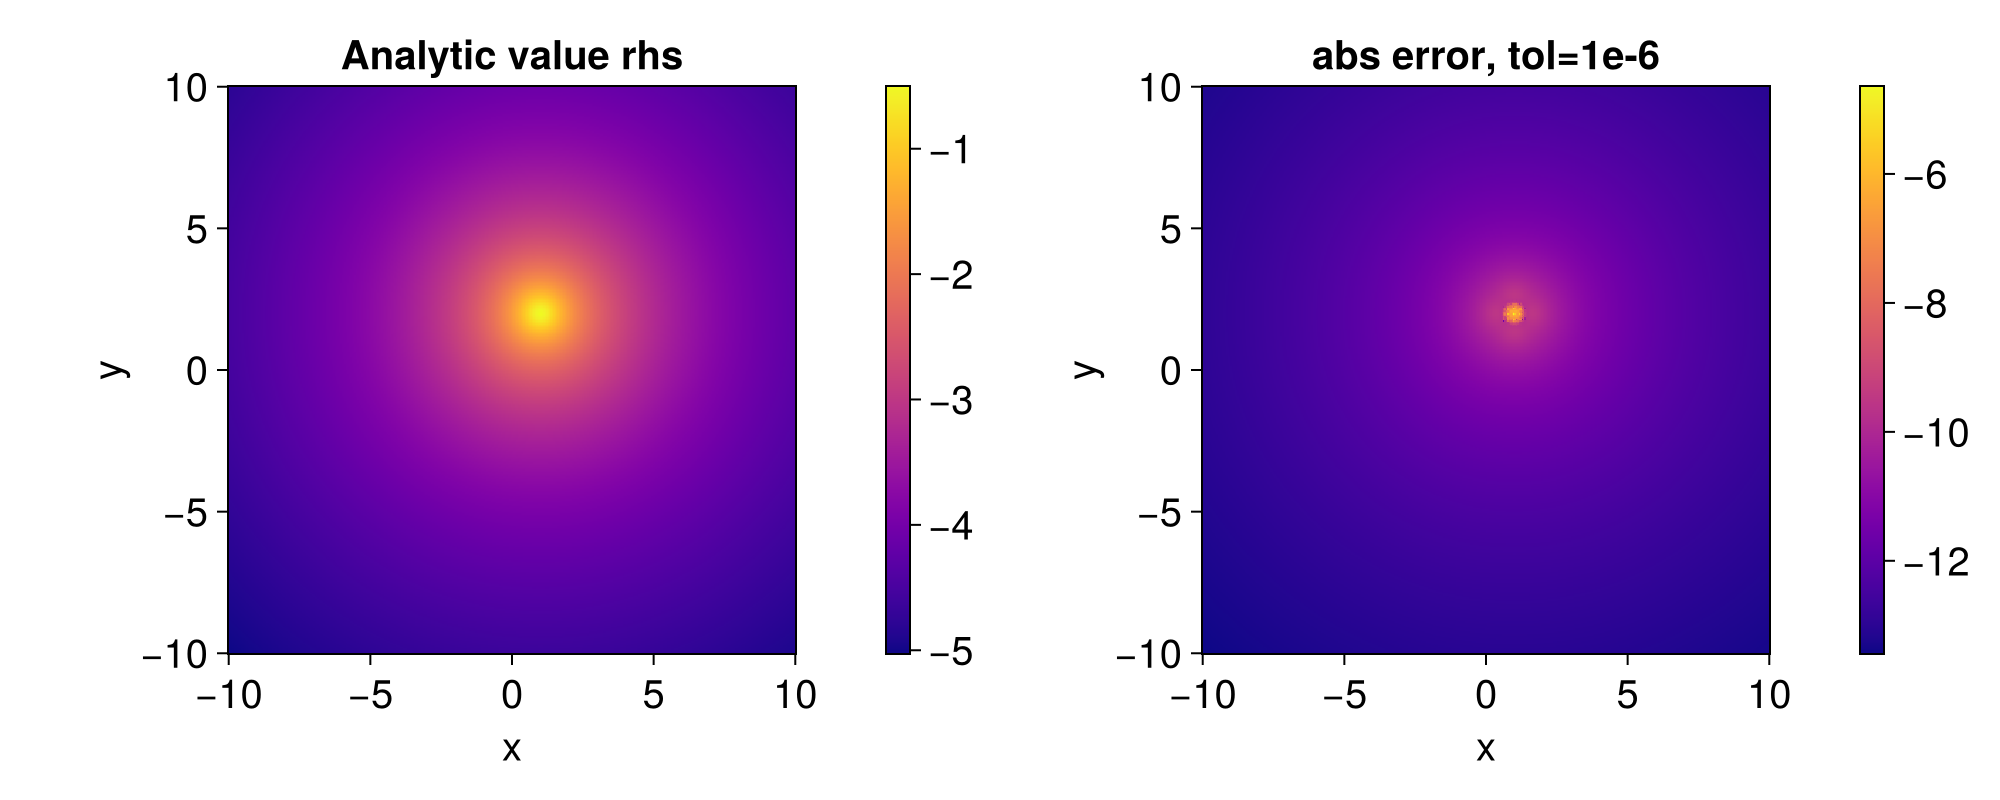
\includegraphics[width=0.95\textwidth]{../codes/volume_source/figs/rhs_accuracy.png}
    \caption{Error of the TKM volume solver for the incident potential \(u_{\mathrm{inc}}\) against direct summation with the sampling points.}
    \label{fig:tkm}
\end{figure}

\subsection{Source-adaptive refinement for target evaluation}\label{sec:postrefine}

The last step is to evaluate the contribution of the layer potential to the target integral
\begin{equation}
    \begin{split}
        V_{ijkl} &= int \rho_{ij}(x)\,u(x)\,\mathrm{d}x \\
        & = \frac{1}{4\pi} \int \int_\Gamma \rho_{ij}(x) \left(  \frac{\sigma(x')}{\abs{x-x'}}\, \mathrm{d}S(x') \right) \mathrm{d}x.
    \end{split}
\end{equation}
for a fixed layer density~$\sigma$ and many target desnities $\rho_{ij}$ (about $10^3$), where each of them takes a large number of target points (about $10^6$ ).
This stage is different from the near-field treatment in Section~\ref{sec:nearfield}: the BIE has already been solved, so we no longer need to preserve a small set of Nystr\"om unknowns.
Instead, for a fixed layer density~$\sigma$, we refine the source panels to accelerate repeated evaluations on many target points.

More precisely, for each source panel $P$ and target density $\rho$, if
\begin{equation}
    d(P,\mathrm{supp}\,\rho) < 5h_P,
\end{equation}
then the panel is dyadically subdivided, and this subdivision is repeated until the refined panel size satisfies
\begin{equation}
    \abs{P^\prime} \le h_0,
\end{equation}
where $h_0$ is a prescribed evaluation-stage threshold.
The resolved layer density is transferred from the original Nystr\"om grid to the refined panels by tensor-product barycentric interpolation.

The purpose of this post-refinement is to move most source--target interactions back into the far-field regime.
After refinement, most target points $y_m$ satisfy $d(y_m,P') > 5h_{P'}$ for the refined panels $P'$, so their contributions can be evaluated efficiently by FMM.
Only the small residual set of genuinely near interactions must still be treated by brute-force quadrature such as \mbox{HCubature}~\cite{HCubature}.
Thus, unlike the near-field correction in Section~\ref{sec:nearfield}, this strategy increases only the evaluation-stage discretization and reduces the cost of repeated target evaluations.

\subsection{Algorithm Summary}

We collect the components described in Sections~\ref{sec:bie}--\ref{sec:tkm} into a
complete procedure for evaluating the four-index integral $V_{ijkl}$, summarized in
Algorithm~\ref{alg:main}.
Each step is detailed below.

\begin{algorithm}[H]
\footnotesize
\algrenewcommand\algorithmicindent{1.2em}
\algrenewcommand\algorithmicrequire{\textbf{Input:}}
\caption{Adaptive BIE solver for the four-index integral $V_{ijkl}$.}
\label{alg:main}
    \begin{algorithmic}[1]
        \Require pair densities $\rho_{ij}$, $\rho_{kl}$; permittivities $\{\epsilon_k\}$;
                interface $\Gamma$; quadrature order $p$; tolerance $\varepsilon$; edge refinement size~$\delta$;  minimum panel size $h_0$
        % \Ensure  $V_{ijkl} = \int \rho_{ij}(x)\,\phi_{kl}(x)\,\mathrm{d}x$
        \State \textbf{// Step 1: incident potential and RHS} \Comment{Sec.~\ref{sec:tkm}}
        \State compute $u_{\mathrm{inc}}$ and $f := -\partial_{\V{n}}u_{\mathrm{inc}}|_{\Gamma}$ via TKM--FFT in Eq.~\eqref{eq:tkm_convolution}
        % \If{$\mathrm{supp}\,\rho_{kl} \subset \Omega_m$}
        %     \State compute $u_{\mathrm{inc}}$ and $f := -\partial_{\V{n}}u_{\mathrm{inc}}|_{\Gamma}$
        %            via TKM--FFT
        % \Else
        %     \State smooth $\epsilon \to \tilde{\epsilon}$ via erf transition (hybrid model)
        %     \State compute $u_{\mathrm{inc}}$ and $f$ with $\tilde{\epsilon}$ via TKM--FFT
        % \EndIf
        \State \textbf{// Step 2: adaptive discretization of $\Gamma$} \Comment{Sec.~\ref{sec:quadrature}}
        \State partition $\Gamma$ into flat panels; equip each with $p{\times}p$ GL quadrature nodes
        \State dyadically subdivide every panel until they satisfy Eq.~\eqref{eq:refine_criterion}; refine panels near edges until $\abs{P} < \delta$
        \State \textbf{// Step 3: assemble and solve the BIE}
        \State set $\mathbf{f} = (f(x_i))_{i=1}^{N}$;\quad
            $(\M{\Gamma})_{ii} = \gamma(x_i)$
        \State define matvec $A\mathbf{v}$ via Eq.~\eqref{eq:nearfield_corrected_A}: near pairs
            ($\abs{x_i{-}x_j}\leq 5h_{P}$) by upsampling correction (Sec.~\ref{sec:nearfield}); far pairs by FMM
        \State solve $A\,\boldsymbol{\sigma} = \mathbf{f}$ by GMRES
        \State \textbf{// Step 4: post-refinement for evaluation}
            \Comment{Sec.~\ref{sec:postrefine}}
        \State subdivide every panel $P$ with $d(P,\mathrm{supp}\,\rho) < 5h_P$
               until $\abs{P} \leq h_0$;
        \State interpolate $\boldsymbol{\sigma}$ to refined panels via
               tensor-product barycentric interpolation
        \State \textbf{// Step 5: evaluate $\phi_{kl} = u_{\mathrm{inc}} + u$ and contract}
        \State far pairs:
               $u(y_m) \mathrel{+}= \tfrac{1}{4\pi}\sum_{i\in P_j}
               \sigma(x_i)\,w_i/\abs{y_m{-}x_i}$ \quad via FMM
        \State near pairs:
               $u(y_m) \mathrel{+}= \int_{P_j} \sigma(x)/({4\pi\abs{y_m{-}x}})\,
               \mathrm{d}S(x)$ \quad via brute force quadrature
        \State \Return $V_{ijkl} \gets
            \sum_m \rho_{ij}(y_m)\,(u_{\mathrm{inc}}(y_m){+}u(y_m))\,w_m^{\mathrm{vol}}$
    \end{algorithmic}
\end{algorithm}

% \paragraph{Step 1: Source preparation and incident potential}
% Given the pair density $\rho_{kl}$, we compute the incident potential $u_{\mathrm{inc}}$ and the right-hand side $f := -\partial_{\V n}u_{\mathrm{inc}}$ at the interface quadrature nodes.
% When $\mathrm{supp}\,\rho_{kl} \subset \Omega_m$, both quantities are evaluated by the TKM--Fourier solver described in Section~\ref{sec:tkm}.
% % When $\rho_{kl}$ straddles a dielectric interface, the permittivity is replaced by the smooth erf-based approximation $\tilde{\epsilon}$ for the evaluation of $u_{\mathrm{inc}}$ only; the sharp interface is retained in the BIE~\eqref{eq:sl} (hybrid model).

% \paragraph{Step 2: Adaptive discretization of the interface}
% The interface $\Gamma$ is partitioned into flat rectangular panels, each equipped with a $p\times p$ tensor-product Gauss--Legendre rule.
% Starting from a coarse partition, we dyadically refine panels according to the RHS-driven and geometry-driven criteria in Eq.~\eqref{eq:refine_criterion}; see Section~\ref{sec:quadrature}.

% \paragraph{Step 3: Assembly and solution of the discrete BIE}
% The Nystr\"om discretization yields the linear system in Eq.~\eqref{eq:linsys}, where the far interactions are handled by FMM and the near interactions by the sparse correction matrix $D^T_{\mathrm{corr}}$ described in Section~\ref{sec:nearfield}.
% The resulting second-kind system is solved iteratively by GMRES.

% \paragraph{Step 4: Source-adaptive mesh refinement for evaluation}
% After solving for $\sigma$, we construct a post-refined source discretization adapted to the target density $\rho_{ij}$, as described in Section~\ref{sec:postrefine}.
% Panels close to the target support are further subdivided, and the resolved layer density is interpolated from the original Nystr\"om grid to the refined panels.
% This step is used only for evaluation, not for the BIE solve.

% \paragraph{Step 5: Potential evaluation}
% Using the post-refined source mesh, we evaluate the scattered potential at the target nodes $\{y_m\}$.
% Most source--target interactions are then treated as far-field and accelerated by FMM, while only a small residual set of genuinely near interactions is evaluated directly.
% The full potential $\phi_{kl} = u_{\mathrm{inc}} + u$ is finally contracted with $\rho_{ij}$ to obtain $V_{ijkl}$.

\paragraph{Complexity}
The dominant cost is the GMRES solve in Step~3, where each iteration costs $\mathcal{O}(N)$ via FMM, giving a total of $\mathcal{O}(N_{\mathrm{iter}}\,N)$.
The iteration count $N_{\mathrm{iter}}$ depends on both the geometry and the permittivity contrast, and can grow as the refinement depth and contrast increase.
% The solver achieves exponential convergence in the refinement depth $n_{\mathrm{adapt}}$, as 
Convergence of the method is going to be demonstrated numerically in Section~\ref{sec:convergence}.

\section{Numerical Results}

In this section, we present numerical studies of the adaptive BIE solver, testing its convergence and accuracy, discussing the edge singularity of the layer density, and demonstrating its application in condensed matter physics.

\subsection{Convergence Study of the BIE Solver}\label{sec:convergence}

\subsection{Edge Singularity}\label{sec:edge_singularity}



\subsection{Application in Condensed Matter Physics}

\section{Conclusion}

\bibliographystyle{elsarticle-num}
\bibliography{ref}

\end{document}
